\section{Results and Discussion}
\label{sec:results}

\subsection{Every Observer Misses the Interior}
\label{sec:blindness}

\begin{table}[t]
\centering
\small
\setlength{\tabcolsep}{3pt}
\caption{\textbf{Every observer misses the interior.} Separation from held-out real
Minecraft houses in each run's own noise floors; GPT-4o rows give the probability that the
judge prefers the real build ($0.5$ is chance). \emph{vis} samples the faces an exterior ray
reaches first and \emph{cut} the faces the cutaway views show. \mvkid{} and \vkid{}:
$n{=}256$ leaderboard, \hollow{} scored against its reference and noise floor; point clouds:
$n{=}128$, seed 0 (\supptab{tab:probe3d}); cutaways: \supptab{tab:ablation}; judge:
\supptab{tab:vlm}.}
\label{tab:observers}
\resizebox{\linewidth}{!}{%
\begin{tabular}{lrrr}
\toprule
observer & \solidify{} & \hollow{} & \matshuffle{} \\
\midrule
\multicolumn{4}{l}{\emph{exterior observation}} \\
\mvkid{}, $4$ views & $\mathbf{+0.35}$ & $\mathbf{+0.04}$ & $+422.43$ \\
Uni3D KID, \emph{vis} & $\mathbf{-0.1}$ & $\mathbf{+0.1}$ & $+19.0$ \\
ULIP-2 KID, \emph{vis} & $\mathbf{-0.1}$ & $\mathbf{-0.1}$ & $+30.6$ \\
chamfer MMD, \emph{vis} & $\mathbf{-0.1}$ & $\mathbf{-0.4}$ & $-0.2$ \\
EMD MMD, \emph{vis} & $\mathbf{+0.0}$ & $\mathbf{+0.0}$ & $-0.0$ \\
GPT-4o, P(real) & $\mathbf{0.53}$ & $\mathbf{0.52}$ & --- \\
\midrule
\multicolumn{4}{l}{\emph{observation that includes the interior}} \\
\mvkid{}, floorplan cuts & $+55.8$ & --- & --- \\
Uni3D KID, \emph{cut} & $+37.0$ & $+13.5$ & $+19.1$ \\
GPT-4o, roof off, P(real) & $0.70$ & $0.73$ & --- \\
\vkid{}, voxel grid & $+444.36$ & $+265.4$ & $+0.00$ \\
\bottomrule
\end{tabular}}
\end{table}

%TL;DR of paragraph: the headline: every observer the field uses misses both interior probes, and each recovers them once its observation includes the interior.
Table~\ref{tab:observers} scores the two interior probes and one appearance control under
every kind of observer the field uses: an image metric on exterior renders, learned and
classical 3D metrics on the surface an exterior ray reaches, and a vision-language judge
shown exterior views. None separates \solidify{} or \hollow{} from real data, and every
one that reads appearance separates \matshuffle{}. Each recovers the interior probes once
its observation includes the interior, and \vkid{}, which reads the voxel grid, separates
them by hundreds of noise floors.

%TL;DR of paragraph: the dose-response curve separates blindness from insensitivity, and raising n does not help.
A metric that is merely insensitive to interiors still moves when the interior changes.
\mvkid{} does not. On the occupancy-noise and mixture axes it is monotone over $185$ and
$549$ noise floors at $n{=}128$. On the interior axis its range end to end is under half a
noise floor, $0.48$ at $n{=}64$ and $0.34$ at $n{=}128$, where \vkid{} reads $133$ and $287$
on the identical rungs of the same dose run (\suppsec{app:tables}). Raising $n$ multiplies the
geometric signal by $2.2$ and leaves the render signal at its sampling floor. Both metrics
rise on the mixture axis, a real arm progressively replaced by bad samples, which is how a
generator actually fails.

%TL;DR of paragraph: all seven render-space statistics miss the probe and catch everything else, so the blindness belongs to the representation.
The flatness is not a property of the one statistic we report. \suppfig{fig:ladder} places
both metrics on eight rungs of known damage in one run, and \supptab{tab:seven} puts seven
render-space statistics on one LEGO ladder. Six of them place the deletion of a fifth of a
structure at $7$--$14$ noise floors and one-minus-recall places it at $1.4$, while none of
them places filling the interior above $2.1$. The blindness belongs to the representation
they read rather than to any one of them.

%TL;DR of paragraph: leaving the image is not enough; a 3D-native metric inherits the null space of what its sampler observes.
Leaving the image does not by itself escape the null space. We score Uni3D, ULIP-2,
chamfer and EMD on point clouds sampled three ways, on our houses and on $290$ multi-room
Objaverse buildings (\suppsec{app:probe3d}). Sampled from the faces an exterior ray
reaches, every point-cloud metric is blind to interior fill and removal, within $1.6$ noise
floors in every cell at both seeds; sampled over all faces, the published default, Uni3D
places a filled Minecraft interior at $+21.7$. Surface-fitted generators emit exterior
shells, on which the two samplers coincide. A metric inherits the null space of what its
sampler observes. Of fourteen structural metrics, including these encoders on
interior-inclusive points and the voxel IoU and chamfer MMD of voxel generation, only \vkid{}
passes every gate, as do generic orbit-averaged occupancy descriptors (\suppsec{app:vkid-robust}), and the voxel metrics rate the filled corpus closer to real than real data
itself (\suppsec{app:headtohead}).

%TL;DR of paragraph: a VLM judge reading the same exterior views shares the null space, and is a third exterior observer rather than ground truth.
An exterior-view judge shares it too. A pre-registered GPT-4o pairwise judge prefers real
over \solidify{} at chance on exterior views and at $0.70$ once the roof is removed. It
agrees with both metrics that \patchstitch{} beats \gabled{} ($0.72$), yet ranks held-out
real sixth of eleven arms, so it is a third exterior observer rather than ground truth
(\suppsec{app:vlm}).

\subsection{It Is the Observation, Not the Encoder}
\label{sec:ablation}

\begin{figure}[t]
\centering
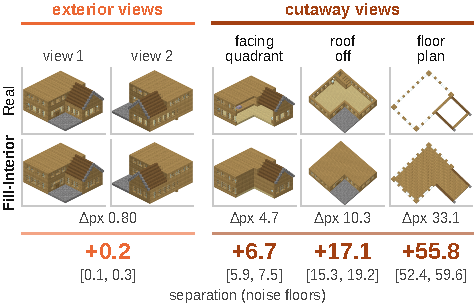
\includegraphics[width=\linewidth]{figures/fig9_cutaway}
\caption{\textbf{The same encoder and statistic, only the views changed.} Each pair is a
held-out build over its \solidify{} twin. \emph{Left:} two of the four exterior views the
standard protocol renders, visually indistinguishable for this build at a mean pixel difference
of $0.8/255$. \emph{Right:} three cutaway protocols on the same builds, each with its separation in
noise floors, with a paired-subsample $95\%$ interval. DINOv2-B,
unbiased KID, $n{=}256$ against $512$ reference builds; full ablation in
\supptab{tab:ablation}.}
\label{fig:cutaway}
\end{figure}

%TL;DR of paragraph: varying encoder, view budget, projection and pooling changes nothing.
The finding could indict DINOv2 at four views rather than render-and-embed as a class. It
does not (Figure~\ref{fig:cutaway}, \supptab{tab:ablation}). Four other encoders, CLIP
ViT-B/16 and B/32, ImageNet-supervised ResNet-50 and the Inception network FID itself uses,
land between $0.0$ and $0.2$ noise floors, as does our DINOv2-B. Eight and sixteen views
covering roof and underside read $+0.2$ and $+0.1$, perspective projection reads $+0.1$, and
face-on elevations, which look straight through windows, read $+4.4$ at $n{=}256$ (\suppsec{app:views25d}).

%TL;DR of paragraph: the cutaway rows are the positive control that makes this a statement about information rather than features.
The cutaway rows are the positive control. The same encoder and the same statistic recover
the interior at $6.7$ to $55.8$ noise floors once the view protocol stops hiding it, which
makes this a statement about \emph{information} rather than about features:
\textbf{the standard view protocol does not put interior structure into the image, so no
encoder downstream of it can score that structure.} A cutaway is not itself a good metric,
because a section view discards the facade the render tier exists to read.

%TL;DR of paragraph: under an opaque renderer the invisibility is exact, which makes it a theorem rather than a measurement.
Under an \emph{opaque} renderer interior damage provably never reaches the image: filling sealed air cannot alter any exterior
view, so no encoder and no statistic can separate it at any sample size. Rendered with
glass opaque, one fixed texture atlas and a CPU rasterizer, all $1{,}596$ test-split views are
bit-identical under both \solidify{} and \hollow{}, so their \mvkid{} separation from real is
exactly $0$; \suppsec{app:hull} gives the proof.

%TL;DR of paragraph: our renderer leaks through glass and an atlas artifact, the leak moves each build's feature in proportion, and the set statistic does not follow it.
Our default renderer is not opaque, and under it \solidify{} alters $\mathbf{91\%}$ of the
$1{,}596$ test-split views, touching a median $1.23\%$ of pixels at a median maximum
channel difference of $\mathbf{128/255}$. Doorways never leak, as air a doorway reaches is
not sealed; glass in front of a filled void does, as does an atlas artifact of our mesh
builder, and with the atlas fixed the fill shows in $67\%$ of houses (\suppsec{app:hull}).
Binned by how much of its silhouette the fill changes, each house's DINOv2 feature moves
in proportion (Spearman $0.96$), yet no bin moves \mvkid{} by more than $1.4$ noise floors:
the leak reaches single images, not the set statistic.

\subsection{Both Directions and Three Domains}
\label{sec:hollow}

%TL;DR of paragraph: hollowing is as invisible as filling, so the blindness runs along the whole interior axis, and separations compare within a run.
The corruption this field actually produces is the converse of \solidify{}: the hollow
shells that surface-fitted mesh and implicit generators emit. It is equally invisible. Against
the leaderboard's reference and noise floor at $n{=}256$, \mvkid{} places \hollow{} at $+0.04$
noise floors and \solidify{} at $+0.35$, while \vkid{} places the same two arms at $+265.4$
and $+444.36$ (\suppsec{app:views25d}). The render metric is blind along the whole interior
axis rather than to one hand-built probe.

%TL;DR of paragraph: the LEGO replication reproduces the qualitative structure, and a published LEGO generator separates on both tiers.
\label{sec:lego}The pattern is not a property of Minecraft houses. On the LEGO corpus
(Table~\ref{tab:lego}, \suppfig{fig:lego}), \mvkid{} places the solidified arm
\emph{below} the real floor and \vkid{} at $\mathbf{+118.6}$, while the render metric
separates \matshuffle{} at $+140.0$ and \monochrome{} at $+685.8$. A published LEGO
generator, BrickGPT \citep{pun2025brickgpt}, prompted with captions of $253$ held-out test
objects, separates on both tiers, $+11.8$ and $+51.5$, beside a solidified control at
$-0.09$ and $+36.4$; its own validity and stability reproduce (\suppsec{app:brickgpt}).

\begin{table}[t]
\centering
\small
\setlength{\tabcolsep}{4pt}
\caption{\textbf{LEGO.} Separation from held-out real in each run's own noise floors.}
\label{tab:lego}
\begin{tabular}{lrr}
\toprule
arm & \mvkid{} & \vkid{} \\
\midrule
\multicolumn{3}{l}{\emph{ShapeNet bricks with a sealed void, $n{=}256$}} \\
\solidify{}    & $\mathbf{-0.01}$ & $\mathbf{+118.6}$ \\
\matshuffle{}  & $+140.0$ & $+0.0$ \\
\monochrome{}  & $+685.8$ & $+0.0$ \\
\midrule
\multicolumn{3}{l}{\emph{StableText2Brick test split, $n{=}253$}} \\
\solidify{}    & $-0.09$ & $+36.4$ \\
BrickGPT \citep{pun2025brickgpt} & $+11.8$ & $+51.5$ \\
\bottomrule
\end{tabular}
\end{table}

%TL;DR of paragraph: the third domain, Objaverse meshes, shows the same split between exterior and interior observation.
On $290$ multi-room Objaverse buildings, the third domain, a DINOv2 kernel distance on four
exterior views reads $+0.0$ for both removing the hidden faces and filling the hidden volume,
at both seeds, while four cutaway views read $9.0$ to $13.7$ and \vkid{} $23.7$ to $118.4$
(\supptab{tab:probe3d}).

\subsection{Complementary Blindness and the Leaderboard}
\label{sec:complementary}

\begin{table*}[t]
\centering
\small
\setlength{\tabcolsep}{3pt}
\caption{\textbf{The leaderboard} ($n{=}256$ per arm, $399$ reference builds). Appearance
and geometry are null-standardized $z$-scores: the arm's distance from held-out real over
the standard deviation of $48$ real-vs-reference draws at this $n$. That deviation shrinks by
a factor of $0.49$ to $0.72$ when $n$ doubles, so the $z$-scores are \textbf{not comparable across $n$}; the raw
MMD$^2$ columns ($\times 10^3$) are stable in $n$. \blockscore{} is the
\textbf{maximum} across five pillars; palette and the two structure pillars never determine
it here, and the structure pillars use a coarser in-run scale (\suppsec{app:blockscore}). Rank is the $95\%$ interval over $1{,}000$ subsample
replicates; an interval spanning several places marks a tie. $\dagger$~marks the contaminated
checkpoint of \suppfig{fig:contamination}, unrankable and shown for comparison. ``Twins'' is
the within-set near-twin rate, the share of builds with a near-copy elsewhere in the same
set ($0.8\%$ for held-out real); its gate disqualifies four rows, whose pillars are shown
for comparison.}
\label{tab:leaderboard}
\begin{tabular}{rlrlrrrr}
\toprule
& & & & \multicolumn{2}{c}{$z$ (noise floors)} & \multicolumn{2}{c}{raw MMD$^2$} \\
\cmidrule(lr){5-6}\cmidrule(lr){7-8}
rank & arm & \blockscore{}~$\downarrow$ & worst pillar & appearance & geometry & \mvkid{} & \vkid{} \\
\midrule
1 & \realheld{} \emph{(anchor)}      & $0.00$   & ---        & $+0.00$   & $+0.00$ & $0.001$ & $-0.14$ \\
\midrule
\multicolumn{8}{l}{\emph{submissions}} \\
$(2)^\dagger$ & \voxar{} \emph{(contaminated)} & $229.29$ & geometry & $+128.87$ & $+229.29$ & $0.208$ & $12.08$ \\
3 & \voxar{} \emph{(clean)}          & $285.22$ & geometry   & $+157.40$ & $+285.22$ & $0.254$ & $15.06$ \\
4 & \voxarun{} \emph{(clean)}        & $345.10$ & geometry   & $+182.86$ & $+345.10$ & $0.295$ & $18.25$ \\
5--7 & \patchstitch{}                & $431.70$ & appearance & $+431.70$ & $+368.21$ & $0.696$ & $19.48$ \\
10 & \randomvox{}                    & $1087.06$ & appearance & $+1087.06$ & $+727.48$ & $1.752$ & $38.63$ \\
\midrule
\multicolumn{8}{l}{\emph{probes and controls: known damage, not submissions}} \\
5--7 & \textbf{\solidify{}}          & $444.36$ & geometry   & $\mathbf{+0.35}$ & $\mathbf{+444.36}$ & $0.001$ & $23.54$ \\
5--7 & \matshuffle{}                 & $422.43$ & appearance & $+422.43$ & $\mathbf{+0.00}$ & $0.681$ & $-0.14$ \\
8 & \monochrome{}                    & $535.36$ & appearance & $+535.36$ & $+0.00$ & $0.863$ & $-0.14$ \\
9 & \copynoise{}                & $619.13$ & geometry   & $+271.94$ & $+619.13$ & $0.439$ & $32.86$ \\
\midrule
\multicolumn{8}{l}{\emph{disqualified: refused a rank, with the reason}} \\
  & Dream-Cubed \citep{merino2026dreamcubed} & DQ & twins $59.8\%$ & $+165.71$ & $+146.64$ & $0.268$ & $7.67$ \\
  & \emph{vanilla village templates} ($n{=}174$) & DQ & twins $67.2\%$ & $+110.21$ & $+202.95$ & $0.178$ & $10.67$ \\
  & \gabled{}                       & DQ & twins $20.7\%$ & $+535.62$ & $+620.98$ & $0.863$ & $32.96$ \\
  & \hollowbox{}                    & DQ & twins $24.6\%$ & $+864.00$ & $+645.86$ & $1.392$ & $34.28$ \\
  & \singlemode{}                    & DQ & \multicolumn{5}{l}{mode collapse, $+44.9$ spreads on voxel diversity} \\
  & \traincopy{}                     & DQ & \multicolumn{5}{l}{memorization, $+10.1$ spreads on retrieval percentile} \\
  & Dream-Cubed \emph{(whole chunk)} & DQ & \multicolumn{5}{l}{mode collapse, $+24.0$ spreads on voxel diversity: every chunk is a slab of terrain} \\
\bottomrule
\end{tabular}
\end{table*}

%TL;DR of paragraph: each tier is fooled by the corruption aimed at it and rescued by the other, and the asymmetry between the two failures is large.
Table~\ref{tab:leaderboard} shows the complementarity directly. \solidify{} reads $+0.35$
on appearance against $+444.36$ on geometry, and \matshuffle{} is the converse, $+422.43$
on appearance against \emph{exactly} $+0.00$ on geometry. Noise floors grow with $n$, so
we compare tiers by effect size, $\sqrt{\text{MMD}^2}$ as a fraction of \randomvox{}'s
under the same metric: \solidify{} sits at $0.03$ on appearance, inside the $0.03$ that
fresh real draws reach, and at $0.78$ on geometry (\suppsec{app:failrate}). Each tier is fooled by the corruption aimed at it and
rescued by the other, which is why \blockscore{} takes the worst pillar. The two failures
differ in severity: the best attack we have on \vkid{}, \patchstitch{}, buys
near-perfect local occupancy statistics with globally incoherent structure and still sits
at an effect size of $0.71$ on geometry. The two feature spaces dissociate build by build as well: asked for each probe's
nearest held-out real build, the render features return a filled house's own source
$100\%$ of the time and \vkid{}'s features $26\%$, and for \matshuffle{} the proportions
reverse, $26\%$ against $100\%$ (\suppfig{fig:nn}).

%TL;DR of paragraph: the published generator is disqualified for repeating itself, which a new within-set gate catches and the train-split gates did not.
Dream-Cubed \citep{merino2026dreamcubed}, the one published generator we score, is
disqualified (\suppsec{app:dreamcubed}). Scored on the largest constructed component of
each terrain chunk its village checkpoint emits, its builds copy nothing from our training
split (duplicate rate $0.004$) but copy each other: $59.8\%$ have a near-copy in the same
set (occupancy IoU $\geq 0.8$ under rotation, mirroring and translation), against $0.8\%$
for held-out real, and they are vanilla village pieces, $36\%$ of them roofless
enclosures. Neither novelty gate saw this, so we added a within-set near-twin gate under
the duplicate gate's rule. It disqualifies Dream-Cubed at $+29.5$ spreads, the two
parametric baselines, and the game's own village templates, which would otherwise score
$202.95$, ahead of every model we trained.

%TL;DR of paragraph: the geometric separation does not come from the added mass or from the sealed-interior scalar.
Deleting \vkid{}'s size term and sealed-interior scalar leaves $197.3$ of its $201.8$
floors on \solidify{} in the protocol run (\suppsec{app:descriptor}). Every leave-one-family-out variant, every random half of its
dimensions and descriptors with no hand design (random 3D CNNs, raw $3^3$ patterns) pass
all gates, the last at $257$ to $437$ floors on \solidify{} (\suppsec{app:vkid-robust}).

%TL;DR of paragraph: a mass-matched control separates on the render metric and not the geometric one, which is the dissociation stated without a probe-specific argument.
The sharper test is a control matched on the quantity in question. \growshell{} dilates the
solid outward until it has added \emph{exactly} the number of blocks \solidify{} adds to
that build, which it achieves to within one block on $128$ of $128$ builds at a median of
$196$. Same builds, same material, same mass, and the only difference is whether the new
mass goes inside or outside. The two metrics then part company completely. In that run
\mvkid{} places \growshell{} at $\mathbf{+102.3}$ noise floors and \solidify{} at
$\mathbf{+0.3}$, while \vkid{} places them at $214.5$ and $201.8$. No block count could
produce that pair of rows.

%TL;DR of paragraph: a required provenance field caught contamination that no statistic saw, and the maximum rule names a different failure for each learned arm.
The $\dagger$ row is our own autoregressive checkpoint, which had trained on $346$ of the
$399$ test builds ($87\%$). No distribution statistic and no memorization gate saw it, at a
duplicate rate of $0.000$; a required split declaration did, and retrained on the clean
split the arm loses its margin over the language-model baselines (\suppsec{app:casestudy}).
Benchmarks in this domain should require that declaration and refuse to rank arms that
cannot make it. The maximum rule also names a different failure for each learned arm: the
clean \voxar{} is geometry-limited, $+285.22$ against $+157.40$ on appearance, and
\patchstitch{} is limited by appearance, so a mean over pillars would hide both.

\subsection{Limitations}
\label{sec:limitations}

%TL;DR of paragraph: what each tier measures, stated as scope: the proof covers opaque rendering, V-KID reads local geometry, and neither tier scores interior appearance.
The invisibility is a theorem about opaque rendering (\suppsec{app:hull}); for translucent
renderers it is a measured attenuation, here on one renderer, and a path tracer sharing no
code with ours is the natural replication. \vkid{} reads local geometry. Global coherence is
a separate axis, which \patchstitch{}, assembled from patches of real builds, exposes by
scoring closer to real than the simple but coherent \gabled{} on both tiers, so it stays a
standing control (\suppsec{app:vkid-robust}). \vkid{} is blind to materials by construction,
and neither tier scores how an interior \emph{looks}: cross-section views see it but rank
arms by texture (\suppsec{app:views25d}), so interior appearance is an open measurement.
Detecting interior change is not ranking interior function: \vkid{} accepts cluttered
interiors, and a walk-through test sides with \mvkid{} on $33$ of $40$ reversed generator pairs (\suppsec{app:functional}).

%TL;DR of paragraph: the noise-floor unit depends on n, and the one published Minecraft generator needs an extraction step.
A noise floor is a run's own statistic and roughly halves when $n$ doubles, so magnitudes
compare within a run ($n{=}256$ for the leaderboard, $128$ elsewhere) and only ranks and
ratios carry across runs (\suppsec{app:nscale}). The generator released with this
corpus \citep{chen2019voxelcnn} reports a cumulative chamfer distance,
which is exactly invariant to our probe (\S\ref{sec:related}).
